% Chapter Template

\chapter{Introduction} % Main chapter title

\label{Chapter1} 

%----------------------------------------------------------------------------------------
%	SECTION 1
%----------------------------------------------------------------------------------------

Software development typically consists of a few phases. Initially, developers write code on their local machines. 
Once their new code works, they'll push it to a (git) server. 
There, the code will be reviewed by colleagues and when everyone is happy the new code is ready to deploy, it will get merged to a 'main' branch.
At this point, the operations team takes over and makes sure the new code is live on the production servers.

There's a lot of manual work involved in this process. Wouldn't it be great if steps can be automated?

\begin{figure}[h!]
	\centering
	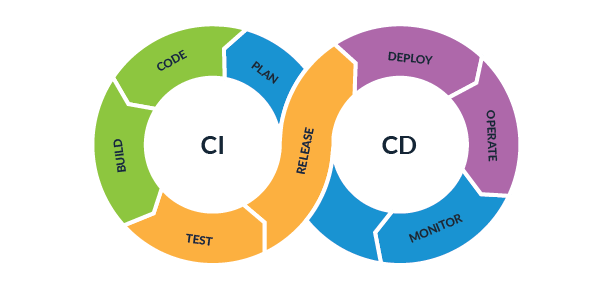
\includegraphics[scale=0.75]{devops}
	\caption{The different phases of DevOps \cite*{devops-8}}
	\label{fig:devops}
\end{figure}


This is where CI/CD (or DevOps) comes in. It is a very broad term but in practice it usually boils down to automating as much as possible and leveraging tools or workflows to achieve that.
In effect, this might mean that during the review phase, the code is automatically compiled and unit tests ran. If the code does not compile, reviewers know instantly that the code is not ready yet.

During continuous integration \cite{Duvall-CI} several components of the software are taken and automated tests are run. 
These tests check things ranging from "does it compile?" to checking business logic and even testing whether or not the entire solution works (End to end testing).

Continuous delivery \cite{Humble-CD} takes this even further. With CD, once the code has been reviewed and is considered ready, scripts will automatically deploy the new code.

By doing this continuously, the friction of these tests and deploying becomes smaller, this significantly reduces the time and effort required to deploy new features.
In practice, it allows teams at large companies like Amazon to deploy \textbf{23.000 times a day}. \cite*{phoenix-project}

Stampix takes advantage of CI/CD in their development workflows.

\section{Initial state}

\begin{figure}[h!]
	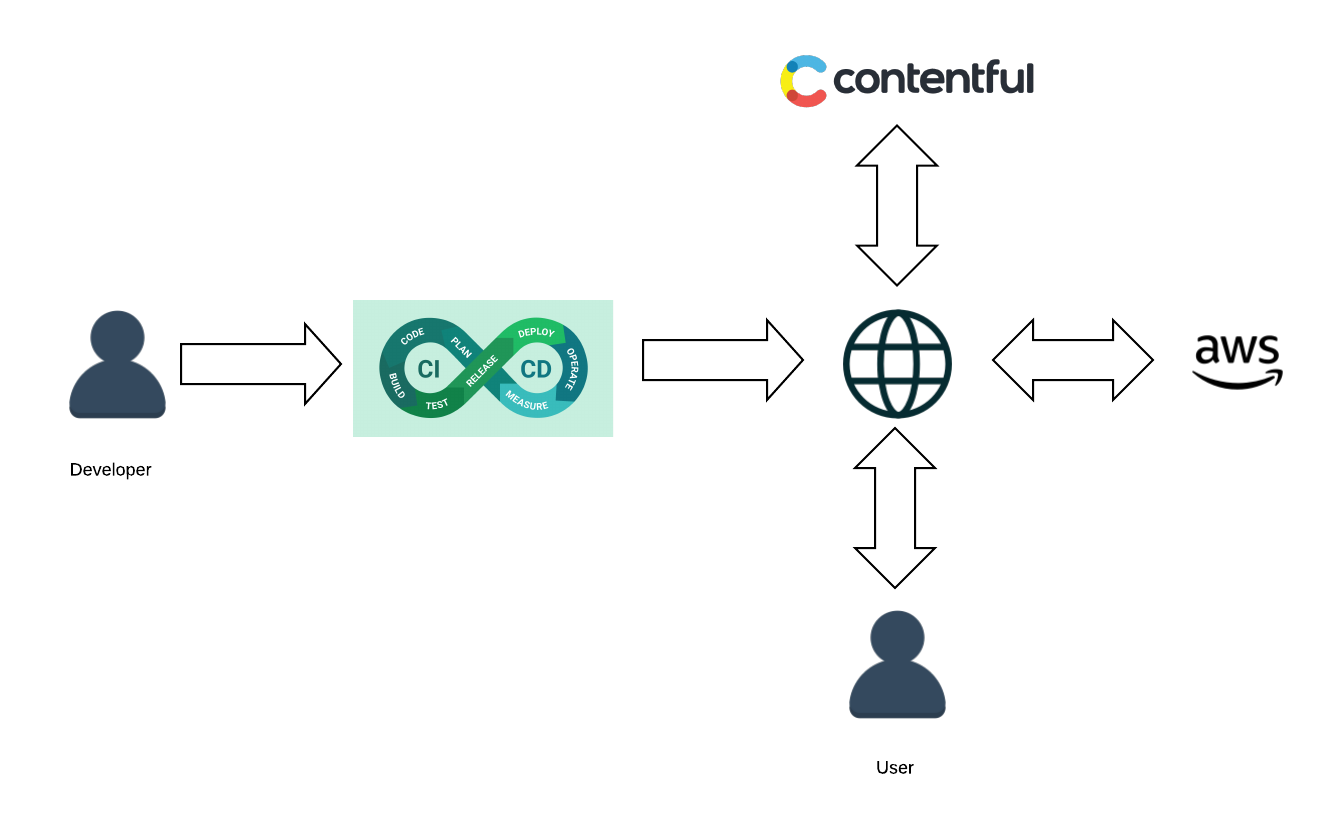
\includegraphics[scale=0.8]{original_flow}
	\caption{The original flow of the web application}
	\label{fig:original_flow}
\end{figure}


The inital state of the process this paper will investigate is a fairly typical web application. 
Developers write code which gets built and deployed by a CI/CD pipeline (1). The result are static files which are served by a webserver.

Users who visit the site receive these static files, after which the application will perform API requests to a CMS which returns the necessary assets (2). 
The application will also send API requests to a backend (hosted on AWS) for completing business logic (3).


\section{Stampix}

This paper was written for Stampix, where I spent a few months doing my internship. During the paper, I will sometimes refer to Stampix as an example or make conclusions in the context of Stampix' business requirements.
Stampix is a startup based in Belgium. It's main clients are businesses, businesses can purchase 'prints' with Stampix which they can then use for marketing/loyalty campaigns. 
The exact purpose always depends on the business, a concrete example would be "Sign up for our newsletter and receive 5 free photos!". So the business is responsible for distributing their purchased prints to the users.

Users who have received these prints can then visit the web application to select photos, crop/rotate/resize/... as needed and ultimately send their selection to Stampix servers. 
At this point, the responsibility of the web application ends and the backend processes take over. The photos are sent to printing partners for printing and distribution.

Stampix has many clients and since the primary use case is using the print for marketing purposes, the web application should be appropriately branded with the clients assets.
